\chapter{Design}
This section will cover the details of the methods and algoithms that were used in the implementation of the project. The previous section covered the history of some of these techniques which were imperative for building the foundation of the methods described in this chapter.

Deep Q-Networks and its enhancements have the majority of focus, as it is the basis of the project. Below is a table of the different experiments and the methods that were used in order to produce the best solution for each tested environment.

\begin{table}[h!]
	\begin{center}
		\begin{tabular}{|c|c|c|}
			\hline
			Network   & Algorithm                  & Environment    \\
			\hline
			CNN + MLP & Q-Learning                 & Pong           \\
			CNN + MLP & Q-Learning                 & Breakout       \\
			CNN + MLP & Duelling Double Q-Learning & Space Invaders \\
			\hline
		\end{tabular}
		\caption{Best performing method in given environment}\label{table:design:algo-experiment}
	\end{center}
\end{table}

\section{Markov decision process}
\label{dsgn:sec:mdp}
This section will describe some of the basics of Markov decision processes (MDP), they are the foundation of the reinforcement learning methods that will be described later in this chapter. First, we need some mathematical definitions of MDPs, these are from David Silver's excellent lecture series on Reinforcement Learning.

Markov decision processes are just markov reward processes with decisions, i.e. At each state $S_t$, we have a finite set of actions to choose from in order to get to a new state $S_{t+1}$.

\begin{defn}
	A Markov decision process is a tuple $\langle \mathcal{S}, \mathcal{A}, \mathcal{P}, \mathcal{R}, \gamma \rangle$.
	\begin{itemize}
		\item $\mathcal{S}$, finite set of states
		\item $\mathcal{A}$, finite set of actions
		\item $\mathcal{P}$, state transition probability matrix,~\\$\mathcal{P}_{ss'}^a = \mathbb{P}[S_{t+1}=s'|S_t=s, A_t=a]$
		\item $\mathcal{R}$, reward function, $\mathcal{R}_s^a = \mathbb{E}[R_{t+1}|S_t=s,A_t=a]$
		\item $\gamma$ discount factor, $\gamma\in[0,1]$
	\end{itemize}
\end{defn}

The definition above defines a Markov decision process, which we use as a basis for describing the methods in reinforcement learning. In order to illustrate the idea, let us consider the game of Pong. For simplicity, assume we can encode each frame of the game into the set of states $\mathcal{S}$. In order to play the game, we need to know what the best action to take would be at each frame of the game to move the paddle under the ball, hitting the ball back and (hopefully) scoring a point.

Given a frame of the game $S_t$ and the set of actions we can choose from $A_t$, we are going to try and maximise our future (expected) reward using the reward function $\mathcal{R}_{S_t}^{A_t}$. We want to choose the best action $a$, that will result in the maximum future reward. It is important that we don't look at immediate rewards only, since, in Pong we don't get the point until we have hit the ball back to the other side.

In order to look at future rewards, we use the discount factor $\gamma$. When $\gamma$ is close to zero, we are ``\textit{myopic}'' in our evaluation (we only look for short-term rewards). However, as $\gamma$ gets closer towards 1, we are ``\textit{far-sighted}'' in our evaluation.

Overall, we need to know a strategy that provides the best action to take in a given state which maximises the expected total reward. This is called a \textit{policy}, denoted by $\pi$.

\begin{defn}
	A \textit{policy} $\pi$ is a distribution over actions given states,
	\begin{center}
		$\pi(a~|~s)=\mathbb{P}[A_t=a~|~S_t=s]$
	\end{center}
\end{defn}

The policy of an agent fully describes the behaviour of the agent (TODO: add ref) which only depends on the current state, not the history. In order to describe the optimal policy for an agent to follow, we first need some more definitions.

\begin{defn}
	$G_t$ is the total discounted reward for time-step $t$
	\vspace*{-7mm}
	\begin{center}
		$$G_t = R_{t+1} + \gamma R_{t+2} + \dots = \sum_{k=0}^{\infty}\gamma^{~k}~R_{t+k+1}$$
	\end{center}
\end{defn}

\begin{defn}
	The \textit{action-value} function $q_\pi(s,~a)$ is expected return starting from state $s$, taking action $a$, following policy $\pi$
	\begin{center}
		$q_\pi(s,~a)=\mathbb{E}_\pi[G_t~|~S_t=s,~A_t=a]$
	\end{center}
\end{defn}

\begin{defn}
	The \textit{optimal action-value} function is denoted by $q_*(s, a)$ and is the maximum action-value function over all possible policies
	\vspace*{-7mm}
	\begin{center}
		$$q_*(s,~a)=\max_\pi q_\pi(s,~a)$$
	\end{center}
\end{defn}

Once we have found the optimal action-value function we consider the MDP ``solved''. Additionaly, we know that we can, given some state, take actions that will lead to the highest possible future reward.

\subsection{Markov property}
With Markov decision processes we assume that in each state, we have all the information we require in order to produce an optimal action. However, in games such as Pong and Breakout, we may not necessarily have all the information we require at a single time. For example, Figure \ref{fig:breakout-brick-fig} shows a screenshot of the Atari game Breakout. In this situation, we cannot decern the optimal action given only this frame as the ball has only just hit the brick.

\begin{figure}[htbp]
	\centering
	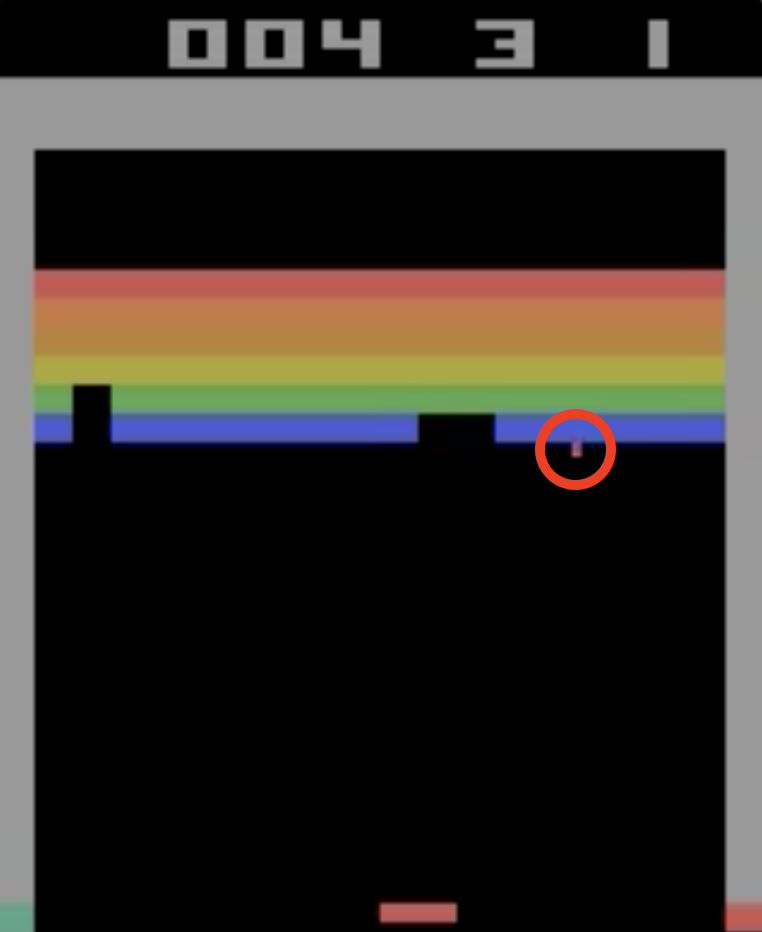
\includegraphics[width=0.30\textwidth]{chapters/chapter3/images/breakout.png}
	\caption[Screenshot of single breakout frame]{Screenshot of a breakout frame with the ball highlighted showing it just before the brick is destrotyed. The ball is highlighted using a red circle.
		\label{fig:breakout-brick-fig}
	}
\end{figure}

In order to solve this problem, in we store a small rolling history of $k$ states (where typically, $k = 4$) called the ``\textit{frame-stack}''. During forward passes through the network we pass the whole frame-stack to the network. This provides a history of frames to the network which has been shown, experimentally, to improve the learning of the algorithm.

\section{Reinforcement learning}
\label{dsgn:sec:rl}
Following on from the previous section on Markov decision processes, this section decribes Reinforcement learning and how these two methods are tightly connected to each other.

In its basic form, RL can be modelled graphically as shown in Figure \ref{fig:rl-diagram}. The agent gets the state from the environment, using its policy, it chooses an action to take -- updating the environment. The environment then produces some new state and a reward signal which the agents uses the pick the next action.

\begin{figure}[htbp]
	\centering
	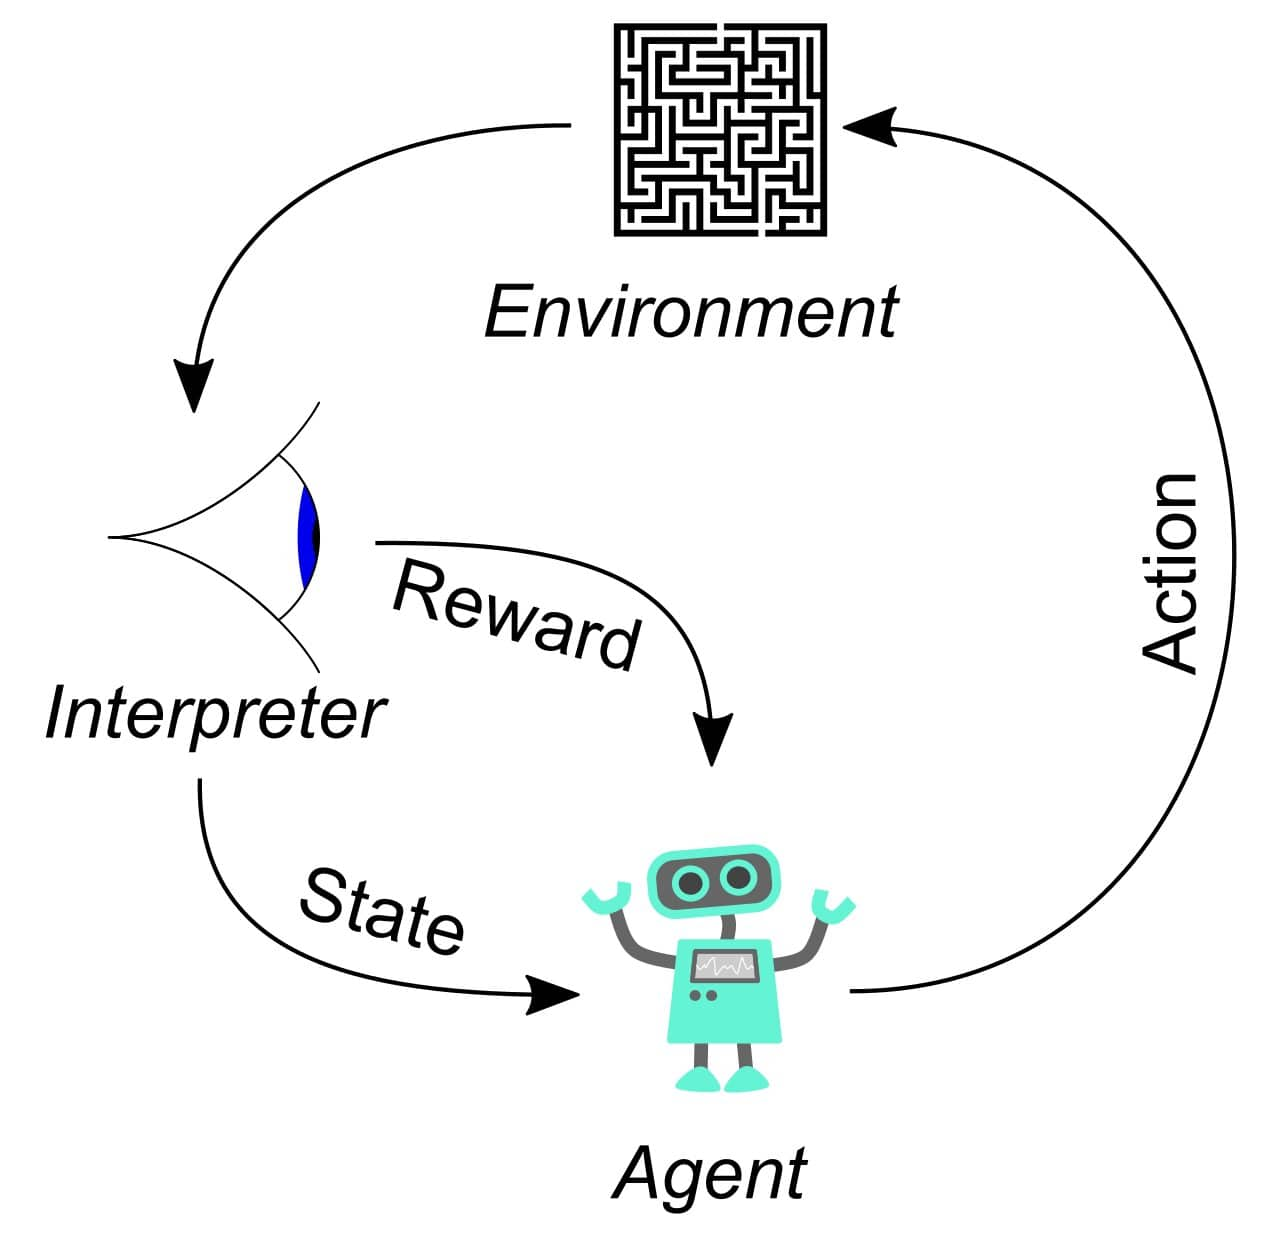
\includegraphics[width=0.35\textwidth]{chapters/chapter3/images/rl.jpg}
	\caption{Diagram of reinforcement learning
		\label{fig:rl-diagram}
	}
\end{figure}

\subsection{Exploration vs Exploitation}
\label{dsgn:sec:rl:expt-v-explor}
A key idea in RL is the problem of exploration vs exploration. This means that if we have an ennvironment, and a policy that dictates how we should navigate the environment, should always follow the policy, or should we deviate and try to find a better path resulting in a higher reward.

In this project we follow a method called $\epsilon$-greedy in which we explore forever, but with a linearly decreasing probability (denoted by $\epsilon$) of random actions, this is decreased over a predefined number of timesteps. Below is the method for choosing the actions.

\begin{center}
	\begin{itemize}
		\item Choose random action with probability $\epsilon$
		\item With probability $1 - \epsilon$ select \vspace*{-9.25mm} action = $$\argmax_{a \in \mathcal{A}}~\hat{Q}(a)$$
	\end{itemize}
\end{center}

Although $\epsilon$-greedy is one of the simplest and a naïve method, it is suprisingly effective in exploring the environment and produces high scoring models. In fact, this method was used in the original DQN paper by V.Mnih et. al. in which they scored better than human averages in the majority of Atari 2600 games.

In the area of reinforcement learning, there are some more advanced methods such as Upper Confidence Bounds (UCB) and Thompson Sampling. However, these Bayesian-based methods are not implemented/explored in this project and is left for future work.

\section{Q-Learning}
\label{dsgn:sec:qlearning}
Q-Learning is a model-free algorithm that is used to solve, iteratively, the Bellman equation for the MDP. By model-free we mean that the algorithm does not require a model of the environment, therefore it can easily handle stoachastic rewards. The method was introduced in 1989 by Chris Watkins in his PhD thesis titled ``\textit{Learning from delayed rewards}''.

We can use Q-Learning in order to approximate $q_*(s, a)$, this produces the optimal policy $\pi$ based on the Q-values. The Q-Learning algorithm stores the state-action values in a large table of values, as represented below in Table \ref{table:design:qtable}. For each possible state that the enviroment can produce, we store a single value (Q-value) for each action that can be performed in that state. These Q-values represents the `\textit{quality}`'' of being in a state $s$ and taking action $a$.

\begin{table}[h!]
	\centering
	\begin{tabular}{|
			>{\columncolor[HTML]{468291}}c |
			>{\columncolor[HTML]{7EB1BD}}c |
			>{\columncolor[HTML]{EFEFEF}}l |
			>{\columncolor[HTML]{EFEFEF}}l |
			>{\columncolor[HTML]{EFEFEF}}l |
			>{\columncolor[HTML]{EFEFEF}}l |}
		\hline
		\multicolumn{2}{|l|}{\cellcolor[HTML]{EFEFEF}}                           &
		\multicolumn{4}{c|}{\cellcolor[HTML]{4682E6}{\color[HTML]{FFFFFF} Actions}} \\ \cline{3-6}
		\multicolumn{2}{|l|}{\multirow{-2}{*}{\cellcolor[HTML]{EFEFEF}Q-Table}}  &
		\multicolumn{1}{c|}{\cellcolor[HTML]{7AA1E1}{\color[HTML]{FFFFFF} NOOP}} &
		\multicolumn{1}{c|}{\cellcolor[HTML]{7AA1E1}{\color[HTML]{FFFFFF} FIRE}} &
		\multicolumn{1}{c|}{\cellcolor[HTML]{7AA1E1}{\color[HTML]{FFFFFF} LEFT}} &
		\multicolumn{1}{c|}{\cellcolor[HTML]{7AA1E1}{\color[HTML]{FFFFFF} RIGHT}} \\ \hline
		\cellcolor[HTML]{468291}{\color[HTML]{FFFFFF} }                          &
		{\color[HTML]{FFFFFF} 0}                                                 &
		0                                                                        &
		0                                                                        &
		0                                                                        &
		0 \\ \cline{2-6}
		\cellcolor[HTML]{468291}{\color[HTML]{FFFFFF} }                          &
		{\color[HTML]{FFFFFF} 1}                                                 &
		-2.3452                                                                  &
		-1.8375                                                                  &
		-2.3634                                                                  &
		-1.5463 \\ \cline{2-6}
		\cellcolor[HTML]{468291}{\color[HTML]{FFFFFF} }                          &
		{\color[HTML]{FFFFFF} \vdots}                                            &
		\vdots                                                                   &
		\vdots                                                                   &
		\vdots                                                                   &
		\vdots \\ \cline{2-6}
		\multirow{-4}{*}{\cellcolor[HTML]{468291}{\color[HTML]{FFFFFF} States}}  &
		{\color[HTML]{FFFFFF} 128}                                               &
		2.4456                                                                   &
		1.2345                                                                   &
		6.3462                                                                   &
		3.8356 \\ \hline
	\end{tabular}
	\caption[Q-Table Example]{Example of how state-action pairs are stored in a Q-Table (NOOP abbreviates `No action/No operation')}\label{table:design:qtable}
\end{table}

Since the Q-Learning algorithm is iterative, at each timestep, we need to update the Q-value corresponding to the occupied state and the action we took. In Chapter \ref{dsgn:sec:dql} this idea will be expanded upon, by using neural networks as a function approximator, replacing the need to store the whole table of Q-values. Algorithm \ref{algo:qlearning} shows how the algorithm is implemented in order to both, predict the next action to take, and updating the Q-table. In order to update the Q-values for each state we use the Q-value update equation which is shown below.

\begin{defn}
	$$Q(s, a) = Q(s, a) + \alpha(R + \gamma \max_a Q(s_{t+1}, a) - Q(s, a))$$
	\begin{itemize}
		\item $Q(s, a)$, q-value for state-action pair
		\item $\alpha$, learning rate
		\item $R$, immediate reward from enviroment
		\item $\gamma$ discount factor, $\gamma\in[0,1]$
		\item $max_a Q(s_{t + 1},~a)$, estimate of optimal future reward
	\end{itemize}
\end{defn}

A major issue with Q-Learning is that since we perform a maximisation of all future rewards when updating the Q-values, this can lead to the algorithm over-estimating the quality of actions and slowing down the learning. During training, we use the same Q-function in order to both produce the expected maximum action-value of future rewards and, select the best possible action in the current state.

\begin{algorithm}[H]
	\SetAlgoNoLine
	\DontPrintSemicolon
	Initialize action-value function $Q$ with random values\;
	\For{timestep = 1}{
	Initialise S\;
	\While{S is not done state}{
	With probability $\varepsilon$ choose random action $a_t$\;
	Else, pick $a_t = \max_{a}Q(s_t, a)$\;
	Take action $a_t$ and observse reward $r_t$ and state $s_{t + 1}$\;
	$Q(s, a) = Q(s_t, a_t) + \alpha(R + \gamma~max_{a}Q(s_{t + 1}, a) - Q(s_t, a_t))$\;
	Update $s_t = s_{t + 1}$
	}
	}
	\caption{Tabular Q-Learning}
\end{algorithm}

As shown above, we can use Q-learning to find the optimal policy by storing all the $q_*(s, a)$ values. However, in practise we run into a issue with the size of the Q-table in that it quickly becomes too big to store in memory. This issue is especially prevalent for large MDPs such as those from Atari games due to the raw pixel input. In order to handle the high-dimensonal input from the games, we can instead use a function approximator to estimate the values of $q_*(s, a)$. This idea will be developed in Section \ref{dsgn:sec:dql} where RL is combined with Deep Learning.

\section{Deep Learning}
\label{dsgn:sec:dl}
This section will describe the basics used in the project for Deep Learning and some of the techniques used in order to construct the Deep Q-Networks discussed in Section \ref{dsgn:sec:dql}.

\subsection{Multi-layer perceptron (MLP)}
\label{dsgn:sec:dl:mlp}
The main technique that underpins most of the artificial neural networks (ANN) that are used today is how we combine single neurons to for networks of neurons. Figure \ref{fig:neuron} shows how we model an artificial neuron with weights and activation functions, this is supposed to loosely model how neurons work inside the brain. The input connections are acting in place of synapses which connect together to form networks.

\begin{figure}[ht!]
	\centering
	\begin{tikzpicture}[
		init/.style={
				draw,
				circle,
				inner sep=2pt,
				font=\Huge,
				join = by -latex
			},
		squa/.style={
				draw,
				inner sep=2pt,
				font=\Large,
				join = by -latex
			},
		start chain=2,node distance=13mm
	]
	\node[on chain=2]
	(x2) {$x_2$};
	\node[on chain=2,join=by o-latex]
	{$w_2$};
	\node[on chain=2,init] (sigma)
	{$\displaystyle\Sigma$};
	\node[on chain=2,squa,label=above:{\parbox{2cm}{\centering Activate \\ function}}]
	{$f$};
	\node[on chain=2,label=above:Output,join=by -latex]
	{$y$};
	\begin{scope}[start chain=1]
		\node[on chain=1] at (0,1.5cm)
		(x1) {$x_1$};
		\node[on chain=1,join=by o-latex]
		(w1) {$w_1$};
	\end{scope}
	\begin{scope}[start chain=3]
		\node[on chain=3] at (0,-1.5cm)
		(x3) {$x_3$};
		\node[on chain=3,label=below:Weights,join=by o-latex]
		(w3) {$w_3$};
	\end{scope}
	\node[label=above:\parbox{2cm}{\centering Bias \\ $b$}] at (sigma|-w1) (b) {};

	\draw[-latex] (w1) -- (sigma);
	\draw[-latex] (w3) -- (sigma);
	\draw[o-latex] (b) -- (sigma);

	\draw[decorate,decoration={brace,mirror}] (x1.north west) -- node[left=10pt] {Inputs} (x3.south west);
\end{tikzpicture}
	\caption{Schematic the modelling of a single neuron} \label{fig:neuron}
\end{figure}

The artificial neuron takes inputs $x_1 \hdots x_n$ with corresponding weights $w_1 \hdots w_n$. Usually, the bias $b$ is stored in $w_0$ with $x_0 = 1$. During a forward pass of the network we process the input vector \textbf{x} and producing an output $y$. In the center of the figure we have a single node that represents the function to calculate $u$ which is the weighted sum of the input vector \textbf{x} and vector of weights \textbf{w}. The equation to calculate this quantity is $u = \sum_{i=0}^n w_i~x_i$.

Finally, each neuron has an activation function associated, there are many possible options for these functions such as Logistic (Sigmoid), TanH and ReLU. Each of these functions defines a threshold for when the output $u$ results in a 1/0 output in $y$.

\begin{figure}[ht!]
	\centering
	\adjustbox{scale=0.65}{
		
\begin{tikzpicture}[
		plain/.style={
				draw=none,
				fill=none,
			},
		net/.style={
				matrix of nodes,
				nodes={
						draw,
						circle,
						inner sep=10pt
					},
				nodes in empty cells,
				column sep=2cm,
				row sep=-9pt
			},
		>=latex
	]
	\matrix[net] (mat)
	{
	|[plain]| \parbox{1.3cm}{\centering Input\\layer} & |[plain]| \parbox{1.3cm}{\centering Hidden\\layer} & |[plain]| \parbox{1.3cm}{\centering Output\\layer} \\
	& |[plain]| \\
	|[plain]| & \\
	& |[plain]| \\
	|[plain]| & |[plain]| \\
	& & \\
	|[plain]| & |[plain]| \\
	& |[plain]| \\
	|[plain]| & \\
	& |[plain]| \\    };
	\foreach \ai [count=\mi ]in {2,4,...,10}
	\draw[<-] (mat-\ai-1) -- node[above] {Input \mi} +(-2cm,0);
	\foreach \ai in {2,4,...,10}
		{\foreach \aii in {3,6,9}
			\draw[->] (mat-\ai-1) -- (mat-\aii-2);
		}
	\foreach \ai in {3,6,9}
	\draw[->] (mat-\ai-2) -- (mat-6-3);
	\draw[->] (mat-6-3) -- node[above] {Ouput} +(2cm,0);
\end{tikzpicture}
	}
	\caption{Diagram representation of MLP} \label{fig:mlp}
\end{figure}

Figure \ref{fig:mlp} shows the structure of an MLP (also called artificial neural network), we construct this network by combining multiple neurons together. The MLP consists of the $n$ input neurons (each having a single input value), with then at least one hidden layer. The last hiddenn layer is connected to the output node/nodes.

In general, for each node in the ANN, it will be connected to every other node in the following layer, whether that is another hidden layer or the output layer. This network structure is referred to as ``\textit{fully connected}'' as every node in a layer is connected to every other node in the next layer. One downside to this `fullyconnected-ness' is that it tends to make them prone to overfitting to the input. Therefore, many techniques have been developed in order to reduce overfitting. Some examples are using regularizaition, dropout layers \footnote{Dropout layer. A layer in a ANN that randomly ignores the input from the previous layer with a given probability. It aids in preventing neurons from becoming dependent on other neurons in previous layers, thereby reducing the effect of overfitting.}, early stopping and batch normalisation. This is not the only type of network consisting of artificial neurons; by connecting the neurons in different ways the networks exhibit different behaviours such as recurrennt neural networks (RNNs) that have a small `memory' capacity due to the network structure.

\subsection{Convolutional Neural Network (CNN)}
\label{dsgn:sec:dl:cnn}
Neural networks are excellent approximators for complex functions that need to be learnt, however, when we have high-dimensonal inputs the size of the network can become too difficult to manage. An important note is that any CNN can in theory be implemented as a neural network individual neurons. However, if we take as an example a single frame from Atari which is 210 x 160 pixels each with RGB values. This results in having over 100,000 weights on just the input layers and as such, too many weights to process in an efficient manner.

\begin{figure}[htbp]
	\centering
	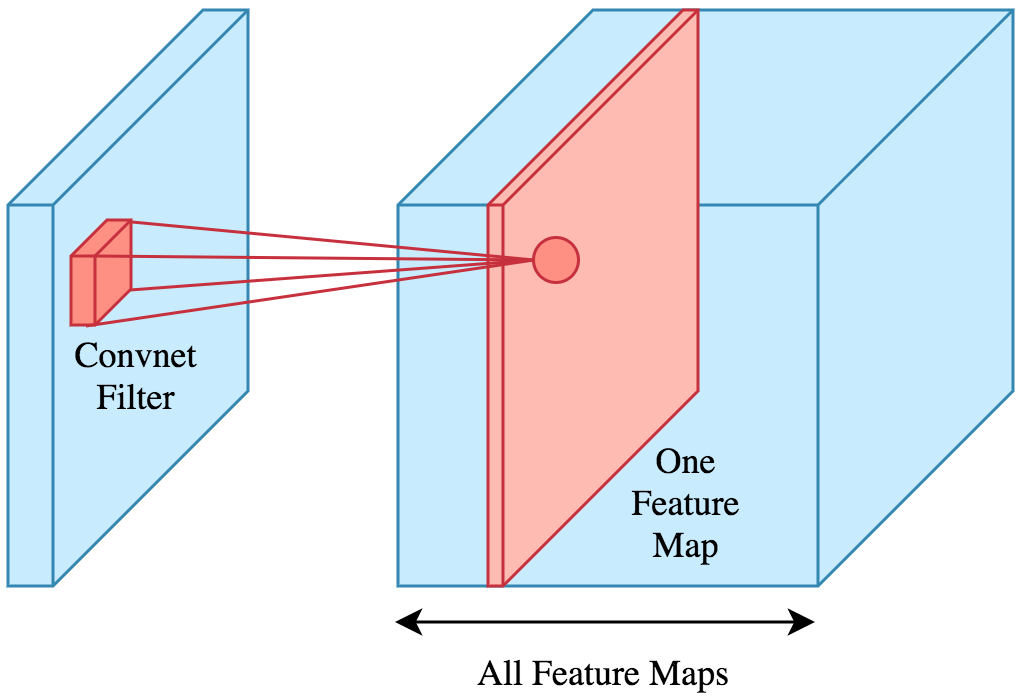
\includegraphics[width=0.5\textwidth]{chapters/chapter3/images/cnn.png}
	\caption{Single convolutional layer using filters
		\label{fig:single-cnn-layer}
	}
\end{figure}

In addition, CNNs can exploit the spatial structure of the data by using different building blocks in order to construct the network. Some of the layers help to avoid problems such as overfitting which is a key problem when training these networks. Others such as ReLU layers help reduce the training time since it simplifies the activation functions with having too much impact on the overall network accuracy. Below is a list of a the most common layers used in CNNs with a short explanation the role of each.

\begin{itemize}
	\item Dropout.
	\item Convolutional
	\item Pooling
	\item ReLU
	\item Fully-connected
\end{itemize}

By carefully combining these different layers, we form a convolutional neural network. The main applications are in image recognition and visual processing such as images and video; in this project we a CNN is used to process frames from Atari. As previously touched upon in Section \ref{bg:sec:cnn-vis}, we can view what information the network has chosen to learnt by looking at the activation in each layer, and each filter. It can provide insight into how well the network is learning and if it requires fine-tuning. Figure \ref{fig:mnist-arch} provides an example network that is used to predict the value of a hardwritten digit from the MNIST\footnote{\href{http://yann.lecun.com/exdb/mnist/}{MNIST}. Large database of 60,000 training image of 28x28 images showing hardwritten digits from 0-9} dataset.

\begin{figure}[htbp]
	\centering
	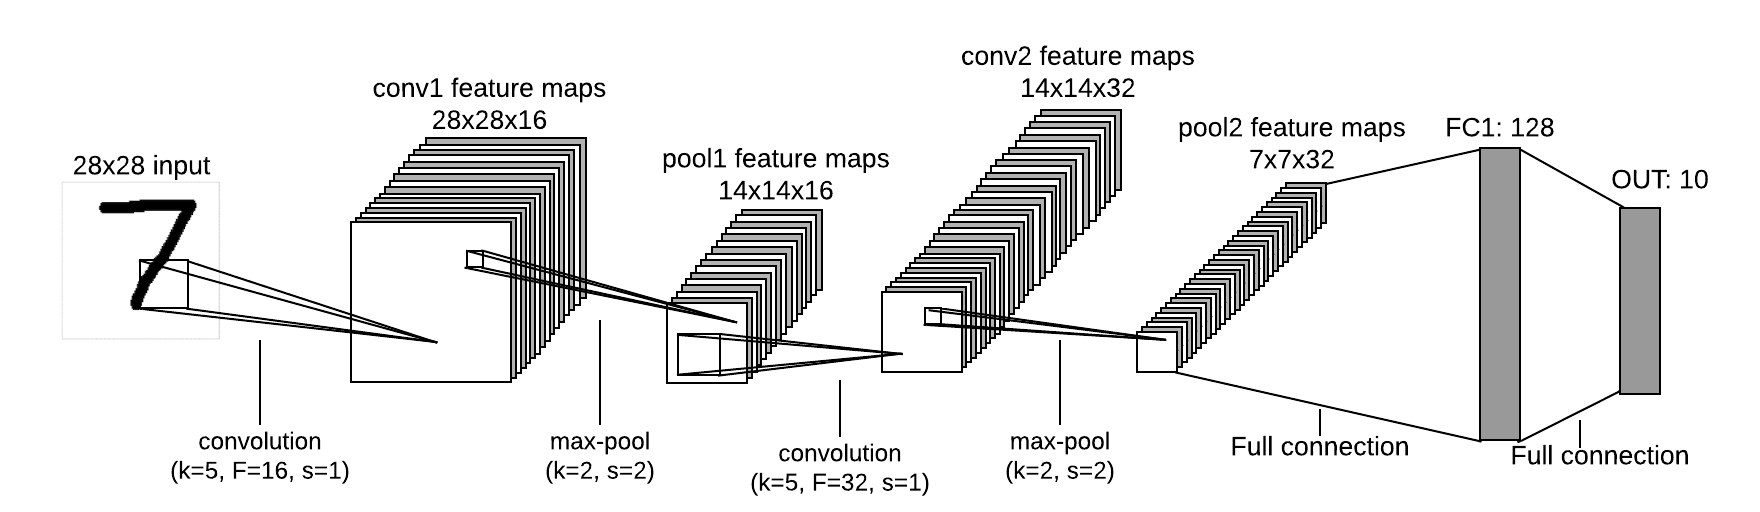
\includegraphics[width=0.65\textwidth]{chapters/chapter3/images/mnist.png}
	\caption{Architecture of a network to predict MNIST digits
		\label{fig:mnist-arch}
	}
\end{figure}


\section{Deep Q-Learning}
\label{dsgn:sec:dql}
\subsection{Experience Replay}

\section{Q-Learning improvements}
\label{dsgn:sec:qlearning:qextra}
Due to the nature of how Q-learning works, it can lead to ann overestimation of the quality of some actions. Therefore, we need a way to help improve the stablity of the algorithm by reducing this overestimation. This section describes two different approaches in order to improve upon the algorithm annd reduce the maximisation bias.

\subsection{Double Q-Learning}
\label{dsgn:sec:qlearning:doubledqn}

\subsection{Duelling Q-Learning}
\label{dsgn:sec:qlearning:dueldqn}
